\documentclass[a4paper, 12pt]{article}

\usepackage[portuges]{babel}
\usepackage[utf8]{inputenc}
\usepackage{amsmath}
\usepackage{indentfirst}
\usepackage{graphicx}
\usepackage[colorinlistoftodos]{todonotes}
\usepackage{natbib}
\usepackage{xcolor}


\begin{document}

\begin{titlepage}
	\begin{center}

\vspace{10pt}
\begin{figure}[!ht]
\centering

\includegraphics[scale=0.2]{img/logo_university.png}
\end{figure}


\huge{Universidade Federal de Pernambuco}
\huge{Centro de Informática}

        
        \vspace{75pt}
        
		\textbf{\LARGE{Aprendizado de Máquina para Reconhecimento de Gestos Manuais Aplicado à LIBRAS (Linguagem Brasileira de Sinais)}}\\
		\vspace{35pt}
		\large{Disciplina: Introdução à Computação - IF668\cite{course}}
		\vspace{60pt}
		
	\end{center}
	
	\begin{flushleft}
		\begin{tabbing}
			Estudantes\qquad\qquad\= Eric Vinícius de Lima\cite{eric}\\
			\>Michel Leonidas Aleixo da Silva\cite{michel}\\
			Professor\> Adriano Lorena Inacio de Oliveira\cite{adriano} \\
			Horário\> Terça-Feira - 10:00-12:00 AM\\
		
	\end{tabbing}
		  
	\end{flushleft}
	
	\begin{center}
		\vspace{25pt}
		Recife, 24 de Outubro de 2021
	\end{center}
\end{titlepage}

%%%%%%%%%%%%%%%%%%%%%%%%%%%%%%%%%%%%%%%%%%%%%%%%%%%%%%%%%%%
\newpage
\tableofcontents
\thispagestyle{empty}

\newpage
\pagenumbering{arabic}

%%%%%%%%%%%%%%%%%%%%%%%%%%%%%%%%%%%%%%%%%%%%%%%%%%%%%%%%%
%%%%%%%%%%%%%%%%%%%%%%%%%%%%%%%%%%%%%%%%%%%%%%%%%%%%
\section{Introdução}

Após uma aula introdutória sobre Aprendizagem de Máquina ministrada pelo Professor Adriano L. I. Oliveira, foi solicitado um projeto com o objetivo geral de aplicar na prática os conhecimentos de Inteligência Artificial. Construindo um programa que envolvesse aprendizado de máquina com modelos baseados em Texto, Imagens, Números ou Sons, aplicáveis a qualquer situação real ou não.

A Linguagem Brasileira de Sinais - LIBRAS - é considerada oficial no país desde 2005 \cite{planalto}, porém, mesmo com mais de 9 milhões de deficientes auditivos (2010) \cite{ibge}, ainda não é ensinada nas escolas públicas, tornando a aprendizagem desta linguagem ainda mais difícil e, consequentemente, a comunicação com o deficiente auditivo.

Com isso, decidimos desenvolver uma aplicação que utiliza Aprendizado de Máquina capaz de julgar com precisão se o gesto feito com a mão é ou não uma vogal pela Linguagem Brasileira de Sinais, através de uma webcam.

\begin{figure}[!ht]
\centering
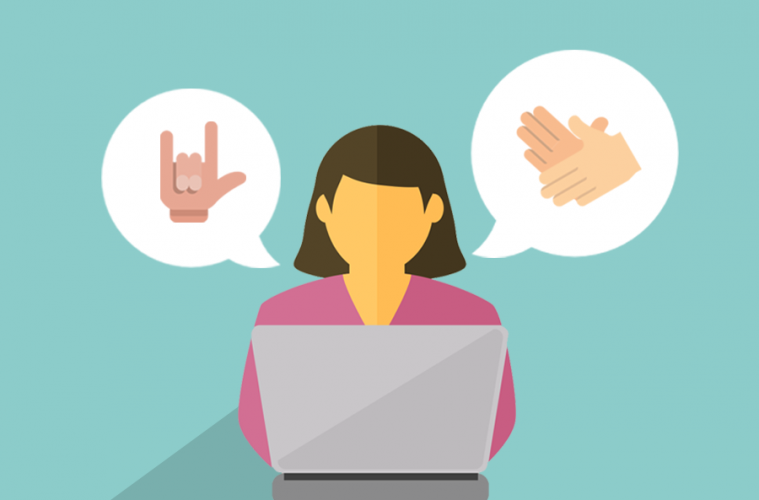
\includegraphics[scale=0.3]{img/inclusion.png}
\caption{Inclusão e acessibilidade de deficientes auditivos\cite{figure_1}}
\label{figure_1}
\end{figure}


%%%%%%%%%%%%%%%%%%%%%%%%%%%%%%%%%%%%%%%%%%%%%%%%%%%%%%%%%%%%%%%
\newpage
\section{Ferramentas Usadas}

Para este experimento, a linguagem de programação Python\cite{python} foi utilizada em conjunto com os frameworks Mediapipe\cite{mediapipe} e OpenCV\cite{opencv}, além da plataforma Machine Learning for Kids\cite{ml4kids} para processamento de resultados com o Watson Assistant da IBM\cite{watson}.

\begin{figure}[!ht]
\centering
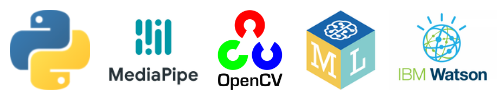
\includegraphics[scale=0.9]{img/tools.png}
\caption{Ferramentas usadas no projeto}
\label{figure_2}
\end{figure}

%%%%%%%%%%%%%%%%%%%%%%%%%%%%%%%%%%%%%%%%%%%%%%%%%%%%%%%%%%%%%%

\section{Procedimento Experimental}

Inicialmente, foi estudado como funciona o reconhecimento de uma mão pelo computador. Normalmente podemos representá-lo computacionalmente como um grafo de 21 vértices. Para reduzir a complexidade, decidimos trabalhar com apenas 11 deles.
 
\begin{figure}[!ht]
\centering
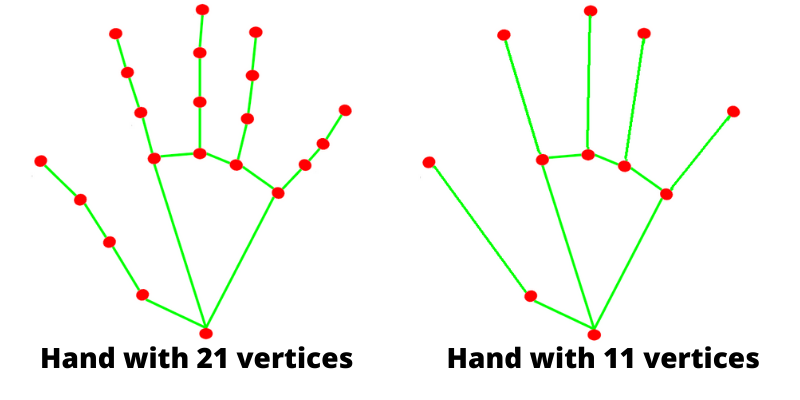
\includegraphics[scale=0.4]{img/hand_vertices.png}
\caption{Mão com diferentes quantidades de vértices}
\label{figure_3}
\end{figure}

Além disso, optou-se por julgar apenas as vogais e não todo o alfabeto em LIBRAS. O Machine Learning for Kids permite que apenas 10 rótulos funcionem com números. Cada vértice possui uma coordenada contendo 2 valores: eixo x e eixo y. Foi então introduzido um impedimento, pelo que decidiu-se reduzir ainda mais o número de vértices, agora para apenas 5. Os vértices mais relevantes foram então escolhidos, seguindo os seguintes gestos:
 
 
 \begin{figure}[!ht]
\centering
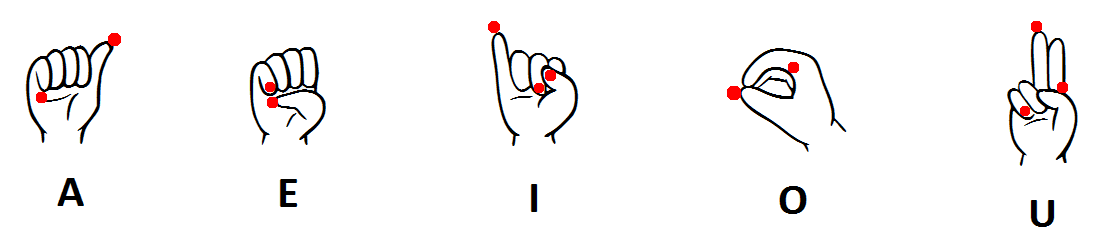
\includegraphics[scale=0.3]{img/hands_gestures.png}
\caption{Vogais em LIBRAS com os principais vértices}
\label{figure_4}
\end{figure}
 
Seguindo a nomenclatura de vértices adotada pelo Mediapipe, os vértices escolhidos foram: 0-wrist, 4-thumb-tip, 5-index-finger-mcp, 12-middle-finger-tip and 20-pinky-tip. Com isso, foi iniciada a elaboração do código do projeto, que foi dividido em 3 partes:



\subsection{Coleta de Dados:}
A primeira parte do projeto foi utilizar as bibliotecas mencionadas para coletar e tratar os dados. O OpenCV foi utilizado para reconhecer uma câmera e realizar algumas configurações de imagem. Em seguida, utilizamos algumas soluções presentes no Mediapipe, para detectar e reconhecer mãos, além de imprimi-las na tela. O MediaPipe trata a mão com 21 vértices, então tratamos esses vértices para pegar apenas 5 deles e removeer o eixo z, pois não é necessário para o projeto.

Por fim, foi possível coletar, por meio de teclas pressionadas no teclado, os eixos x e y de cada um dos vértices escolhidos.

 \begin{figure}[!ht]
\centering
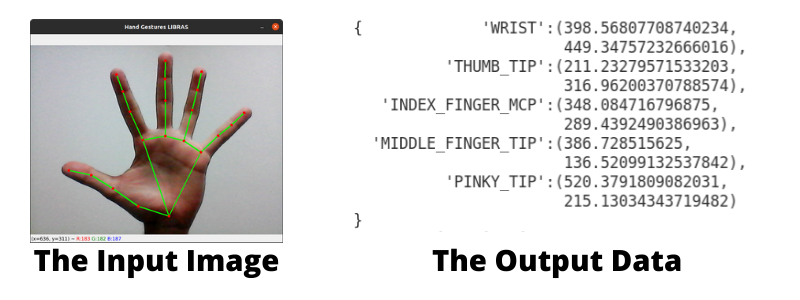
\includegraphics[scale=0.65]{img/data_collect.png}
\caption{Coleta de Dados}
\label{figure_5}
\end{figure}



\subsection{Popular Banco de Dados de Treinamento:}

Para nos comunicarmos com o Machine Learning for Kids, utilizamos sua API, na qual é possível solicitar a classificação dos dados e também o preenchimento do banco de dados de treinamento, e integrá-lo ao projeto através da biblioteca Python Request\cite{requests}. Para isso, foi criado outro módulo responsável por fazer essa comunicação, além de gerar uma chave de acesso API diretamente no Machine Learning for Kids, bem como realizar outras configurações, como a criação de rótulos para as vogais que serão preenchidas.

 \begin{figure}[!ht]
\centering
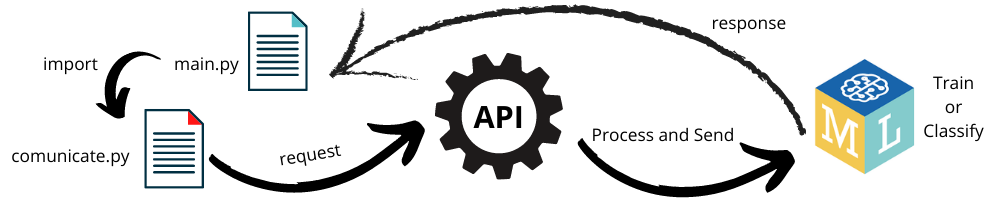
\includegraphics[scale=0.5]{img/api_diagram.png}
\caption{Diagrama da API}
\label{figure_6}
\end{figure}


\subsection{Treinando a Inteligência Artificial:}
Todo o treinamento do computador foi realizado pelo Watson, que utiliza modelos de Rede Neural Convolucional e de regressão linear para classificação. Assim, inicialmente foram adicionados 50 gestos para cada vogal, feitos por pessoas diferentes, com a mão direita e esquerda e em webcams diferentes, para gerar maior precisão nos resultados.

 \begin{figure}[!ht]
\centering
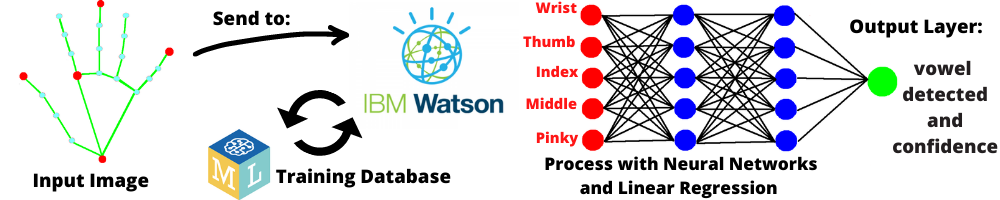
\includegraphics[scale=0.5]{img/training_diagram.png}
\caption{Diagrama do Treinamento}
\label{figure_7}
\end{figure}

O processo de entrada de dados para o banco de dados de treinamento foi automatizado, agora sendo feito pressionando uma tecla do teclado, específica para cada gesto vocálico. E para facilitar a visualização dos vértices principais, optou-se por destacar esses pontos na janela da webcam além de imprimir nesta janela um texto com a o retorno da solicitação efetuada.

%%%%%%%%%%%%%%%%%%%%%%%%%%%%%%%%%%%%%%%%%%%%%%%%%%%%%%%%%%%%
\section{Análise de Resultados:}

Durante a análise dos resultados, que ocorreu em 21/08/2021, o Machine Learning For Kids teve problemas para retornar o percentual de confiança, sempre apresentando 100\% de confiança em todos os testes realizados (corretos e errados). Portanto, para verificar a real confiança desse juiz, foi utilizada a média geral, por meio do número de acertos e erros coletados para cada vogal. Então,os seguintes dados foram coletados:


\begin{table}[h!]
    \centering
    \begin{tabular}{ |c|c|c|c|c| } 
    \hline
    \multicolumn{5}{|c|}{Análise de Resultados - 08/21/2021} \\
    \hline
    Gesto & Testes Feitos & Acertos & Erros & Média de Acertos \\
    \hline
    A & 20 & 12 & 8 & 60\% \\ 
    \hline
    E & 20 & 15 & 5 & 75\% \\
    \hline
    I & 20 & 18 & 2 & 80\% \\
    \hline
    O & 20 & 12 & 8 & 60\% \\
    \hline
    U & 20 & 17 & 3 & 85\% \\
    \hline
    \end{tabular}
    \caption{Análise de Resultados}
    \label{tab:results_analysis}
\end{table}

Percebeu-se que a maior taxa de erro foi com as vogais A e O, uma possível justificativa é que, graficamente, a localização destes pontos é semelhante. Além disso, os erros nas demais vogais ocorreram em maioria quando a mão estava a uma distância maior que um metro da webcam. Portanto, mais 50 gestos foram adicionados ao banco de dados de treinamento (totalizando 100 casos de exemplos por vogal), e novos resultados foram obtidos:

\begin{table}[h!]
    \centering
    \begin{tabular}{ |c|c|c|c|c| } 
    \hline
    \multicolumn{5}{|c|}{Nova Análise de Resultados - 08/22/2021} \\
    \hline
    Gesto & Testes Feitos & Acertos & Erros & Média de Acertos \\
    \hline
    A & 30 & 28 & 2 & 93.3\% \\ 
    \hline
    E & 30 & 29 & 1 & 96.6\% \\
    \hline
    I & 30 & 30 & 0 & 100\% \\
    \hline
    O & 30 & 29 & 1 & 96.6\% \\
    \hline
    U & 30 & 30 & 0 & 100\% \\
    \hline
    \end{tabular}
    \caption{Nova Análise de Resultados}
    \label{tab:results_analysis2}
\end{table}

Com esses resultados mais precisos e com um percentual de acertos acima de 90\%, conclui-se que esta aplicação possui alta confiabilidade no julgamento de vogais da Língua Brasileira de Sinais feitas à mão.

%%%%%%%%%%%%%%%%%%%%%%%%%%%%%%%%%%%%%%%%%%%
\section{Conclusão}

O aprendizado da Linguagem Brasileira de Sinais continuará sendo um desafio não só para os deficientes auditivos, mas também para toda a população. No entanto, aplicativos como este, que são de domínio público, podem servir não apenas para aprender mais sobre o assunto, mas também para inspirar outras aplicações.

A aplicação já se mostrou capaz de cumprir sua função inicial - reconhecer vogais feitas com gestos pela LIBRAS -. Ele usa o Aprendizado de Máquina e, por isso, aprende a cada interação, o que o torna cada vez mais inteligente. Podendo ser utilizado na área de educação, tanto no uso do próprio da aplicação, quanto no ensino de LIBRAS ou no ensino de disciplinas relacionadas ao Aprendizado de Máquina, podendo também ser aprimorado adicionando outro modelo de aprendizado de máquina, adicionando mais vértices, ou até mesmo o fazer em outra linguagem de programação, tornando-o mais acessível para outros públicos.

%%%%%%%%%%%%%%%%%%%%%%%%%%%%%%%%
%  References
\newpage
{\color{white}\section{References}}
\bibliography{ref.bib}
\bibliographystyle{plain}

\end{document}